\chapter{Ergebnisse und Evaluation}\label{chp:ergebnisse}
Die festgelegten Ziele in Abschnitt \ref{chp:Ziele} wurden in der fertig entwickelten Anwendung vollst�ndig erreicht. Um die Qualit�t der Software zu �berpr�fen, wurden eine Reihe von selbst erstellten Testvideos als Eingabe verwendet. Diese Videos wurden bei Bosch in zwei daf�r vorgesehenen R�umen gedreht. Um das entwickelte Programm zu testen, wurden in den Videos einige Szenarien von Personen in verschiedenen Situationen simuliert. Dabei sollte die Software erkennen, ob es sich um eine normale oder au�ergew�hnliche Situation handelt. In einigen Videos haben sich Personen auf den Boden gelegt und sich dann nicht mehr bewegt. In anderen Videos haben sich Menschen auf ein Sofa gesetzt und sind danach darauf eingeschlafen. Dabei wurden die Situation bei Tag und Nacht durchgespielt und bei variierenden Anzahl an Personen im Raum. Dabei konnten die Menschen das Zimmer verlassen und wieder hineinkommen, um zu �berpr�fen, ob sie erneut von der Software erkannt werden. Das Programm hat in allen F�llen gute Ergebnisse geliefert. Die Software konnte dabei nicht jeden Frame der Kamera richtig klassifizieren. Dennoch wurden alle au�ergew�hnlichen Situationen erkannt. Das folgt daraus, dass die au�ergew�hnlichen Situationen erst nach $30$ hintereinander folgenden Frames mit der Klassifizierung \glqq{}$bad$\grqq{} erkannt werden. Es gab somit bei manchen Situationen eine kleine Verz�gerung, bis diese richtig klassifiziert wurden. Auch die Kamera wurde an verschiedenen Orten im Raum positioniert, um die Arbeitsweise der Hintergrundsubtraktion zu untersuchen.\\
Die verwendete Kamera  hat eine Aufl�sung von 1080x720 Pixel und eine Frame-Rate von 15 FPS. Um einer Echtzeitanwendung gerecht zu werden, muss die Software damit mindestens 15 Bilder pro Sekunde klassifizieren und berechnen k�nnen. Dazu wurden einige Tests durchgef�hrt, um die Geschwindigkeit der Berechnung zu bestimmen. Es stellte sich heraus, dass das Programm durchschnittlich 59 Millisekunden pro Bild braucht, um dieses der zugeh�rigen Klasse zuzuordnen und kann somit 16 Frames jede Sekunde klassifizieren. Diese und die folgenden Tests wurden alle auf einem Rechner mit einem Intel i5 3,20 GHz Prozessor und 16 GB RAM.
In der folgenden Abbildung \ref{fig:laufzeit} wurde eine Laufzeitmessung mit 1000 Frames durchgef�hrt. Dabei wurde auf der X-Achse die Nummer des Bildes und auf der Y-Achse die dazugeh�rige Laufzeit abgetragen. Die rote Linie stellt die durchschnittliche Laufzeit dar.

\begin{figure}[H]
	\centering
	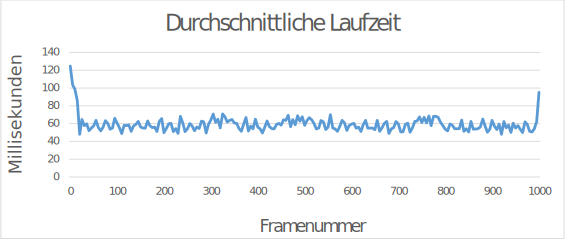
\includegraphics[width=1\textwidth]{fig/laufzeit.pdf}
	\caption{Gemessene Laufzeiten von 1000 Bildern} 
	\label{fig:laufzeit}
\end{figure}

In Abbildung \ref{fig:alarm} wurden drei Videos mit dem Programm untersucht. Die normalen und au�ergew�hnlichen Situationen in diesen Videos sind bereits bekannt. Die Software wurde zum analysieren der Frames verwendet und anschlie�end die Klassifikationen des Programms mit den bereits bekannten Zuordnungen der Bilder verglichen. Die X-Achse nummeriert die Frames und die Y-Achse stellt die Zuordnung des Bildes dar. bei $y=1$ handelt es sich um eine normale Situation und bei $y=0$ um eine au�ergew�hnliche Situation. Die blaue Kurve stellt dabei die richtige bzw. bereits bekannte Zuordnung und die gelbe Kurve die berechnete Klassifikation dar.\\

\begin{figure}[H]
	\centering
	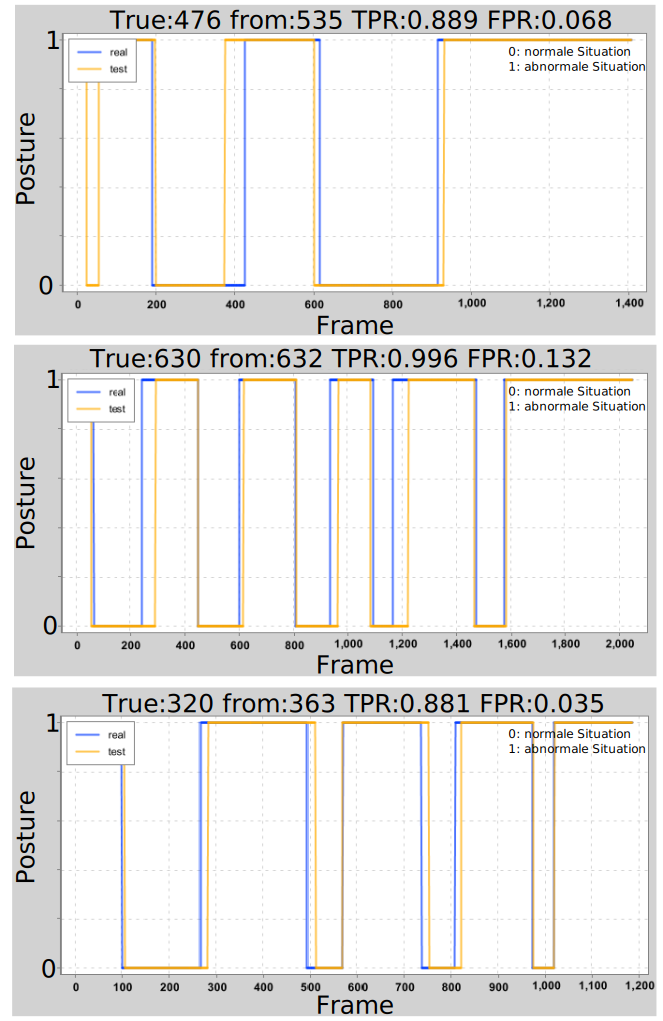
\includegraphics[width=0.9\textwidth]{fig/alarmevaluation2.png}
	\caption{Richtige Zuordnungen (blau) und berechnete Zuordnung (gelb) der Bilder grafisch dargestellt} 
	\label{fig:alarm}
\end{figure}

Nicht alle Frames wurden durch das Programm richtig klassifiziert. Dennoch wurden mehr als $80\%$ der Bilder richtig zugeordnet. Die Erkennung au�ergew�hnlicher Situationen h�ngt dabei nicht von den einzelnen Frames ab. Eine solche Situation wird erst dann erkannt, wenn $30$ Frames hintereinander als au�ergew�hnlich klassifiziert werden. Daher konnte die Software, trotz kleinen Verz�gerungen, alle au�ergew�hnlichen Situationen erkennen.\\
Um eine bessere �bersicht �ber die Zielgenauigkeit des Programms zu schaffen, wurden ROC-Kurven (siehe Abbildung \ref{fig:roc}) mit den implementierten Algorithmen sowie Verbesserungen aufgestellt.

\begin{figure}[H]
	\centering
	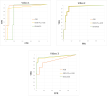
\includegraphics[width=1\textwidth]{fig/ROC2.pdf}
	\caption{ROC-Kurze zur Bewertung des Programms.} 
	\label{fig:roc}
\end{figure}

W�hrend der Entwicklung der Software wurden zwei signifikante Methoden implementiert, um das Programm zu optimieren. Als erstes wurde die ASB-Methode verwendet, die die Hintergrundsubtraktion verbessert. Da sonst zum Beispiel eine stehende Person in einem Raum, die sich lange nicht bewegt, ins Hintergrundbild aufgenommen und nicht mehr als \glqq{}sich bewegendes Objekt\grqq{} erkannt wird. Die zweite Modifikation ist die Kombination von der ASB-Methode und der KNN-Methode. Wobei die KNN-Methode die Genauigkeit der Hintergrundsubtraktion erh�ht. In Abbildung \ref{fig:roc} wird der Unterschied bzw. die Verbesserungen anhand den einzelnen ROC-Kurven dargestellt. Um die Performance weiter zu optimieren, wurde das Bild, vor der Verarbeitung, runter skaliert. Daraus entsteht ein Genauigkeitsverlust, der aber nicht stark genug ist, um die Qualit�t des Programms signifikant zu beeinflussen.



\begin{table}[H]
	\centering
	
	
	\begin{tabular}[H]{|c|c|cc|cc|c|}
		\hline 
		\multicolumn{2}{|c|}{\multirow{ 2}{*}{}} & \multicolumn{5}{c|}{abnormale Situation}\\
		\cline{3-7}
		\multicolumn{2}{|c|}{}& TNR & FNR & TPR & FPR & ACC\\
		\hline
		
		\multirow{ 2}{*}{\rotatebox[origin=c]{90}{{ Video 1 }}} & ASB & 0,869 & 0,037 & 0,962 & 0,0085 & 0,927\\
		
		& KNN-Plus-ASB & 0,762 & 0,11 & 0,889 & 0,053 & 0,917\\
		
		& 854x450 & 0,762 & 0,014 & 0,985 & 0,217 & 0,846\\
		
		\hline
		
		\multicolumn{7}{|c|}{}\\
		\hline
		\multirow{ 2}{*}{\rotatebox[origin=c]{90}{{ Video 2 }}} & ASB & 0,748 & 0,030 & 0,993 & 0,128 & 0,888\\
		
		& KNN-Plus-ASB & 0,763 & 0,024 & 0,996 & 0,111 & 0,903\\
		
		& 854x450 & 0,755 & 0,033 & 0,988 & 0,116 & 0,896\\
		\hline
		\multicolumn{7}{|c|}{}\\
		\hline
		\multirow{ 2}{*}{\rotatebox[origin=c]{90}{{ Video 3 }}} & ASB & 0,805 & 0,058 & 0,763 & 0,080 & 0,795\\
		
		& KNN-Plus-ASB & 0,956 & 0,029 & 0,881 & 0,014 & 0,938\\
		
		& 854x450 & 0,913 & 0,021 & 0,911 & 0,033 & 0,918\\
		\hline
	\end{tabular}
	\caption{Auswertung der verschiedenen Methoden mit ohne Skalierung des Bilds}
	\label{tbl:auswertung}
\end{table}

In Tabelle \ref{tbl:auswertung} sind die Auswertungen von Video 1, Video 2 und Video 3 zu sehen, die als Eingabe f�r die entwickelte Software dienten. Dabei stehen TNR f�r \glqq{}True Negative Rate\grqq{}, FNR f�r \glqq{}False Negative Rate\grqq{}, TPR f�r \glqq{}True Positive Rate\grqq{}, FPR f�r \glqq{}False Positive Rate\grqq{} und ACC f�r \glqq{}Accuracy\grqq{}.